%
% exemplo genérico de uso da classe iiufrgs.cls
% $Id: iiufrgs.tex,v 1.1.1.1 2005/01/18 23:54:42 avila Exp $
%
% This is an example file and is hereby explicitly put in the
% public domain.
%
\documentclass[cic,tc]{iiufrgs}
% um tipo específico de monografia pode ser informado como parâmetro opcional:
%\documentclass[tese]{iiufrgs}
% monografias em inglês devem receber o parâmetro `english':
%\documentclass[diss,english]{iiufrgs}
% a opção `openright' pode ser usada para forçar inícios de capítulos
% em páginas ímpares
% \documentclass[openright]{iiufrgs}
% para gerar uma versão somente-frente, basta utilizar a opção `oneside':
% \documentclass[oneside]{iiufrgs}
\usepackage[utf8]{inputenc}   % pacote para acentuação
\usepackage{times}              % pacote para usar fonte Adobe Times
\usepackage[alf,abnt-emphasize=bf]{abntex2cite}	% pacote para usar citações abnt
\usepackage{graphicx}          % para inserir imagens
%\usepackage{mathptmx}          % p/ usar fonte Adobe Times nas fórmulas

\graphicspath{ {images/} }

\title{Uma análise dos dados de queimada do INPE no Brasil (preliminar)}
\translatedtitle{Using \LaTeX\ to Prepare Documents at II/UFRGS}

\author{Braz}{José Henrique da Silva}
\advisor[Prof.~Dr.]{Schnorr}{Lucas M.}

% a data deve ser a da defesa; se nao especificada, são gerados
% mes e ano correntes
%\date{maio}{2001}

% o nome do curso pode ser redefinido (ex. para TCs)
\course{Curso de Graduação em Ciência da Computação}

% o local de realização do trabalho pode ser especificado (ex. para TCs)
% com o comando \location:
\location{Porto Alegre}{RS}

% palavras-chave
% iniciar todas com letras maiúsculas
%
\keyword{Formatação eletrônica de documentos}
\keyword{\LaTeX}
\keyword{ABNT}
\keyword{UFRGS}

%
% palavras-chave na lingua estrangeira
% iniciar todas com letras maiúsculas
%
\translatedkeyword{Electronic document preparation}
\translatedkeyword{\LaTeX}
\translatedkeyword{ABNT}
\translatedkeyword{UFRGS}

%
% inicio do documento
%
\begin{document}

% folha de rosto
% às vezes é necessário redefinir algum comando logo antes de produzir
% a folha de rosto:
% \renewcommand{\coordname}{Coordenadora do Curso}
\maketitle

% dedicatoria
\clearpage
\begin{flushright}
\mbox{}\vfill
{\sffamily\itshape
``If I have seen farther than others,\\
it is because I stood on the shoulders of giants.''\\}
--- \textsc{Sir~Isaac Newton}
\end{flushright}

% agradecimentos
\chapter*{Agradecimentos}
Agradeço ao \LaTeX\ por não ter vírus de macro\ldots

% sumario
\tableofcontents

% lista de abreviaturas e siglas
% o parametro deve ser a abreviatura mais longa
% A NBR 14724:2011 estipula que a ordem das abreviações
% na lista deve ser alfabética (como no exemplo abaixo).
\begin{listofabbrv}{SPMD}
	\item[API] Application Programming Interface (Interface de Programação de Aplicação)
	\item[CSV] Comma Separated Values (valores separados por vírgulas).
    \item[GMT] Greenwich Mean Time
    \item[INPE] Instituto Nacional de Pesquisas Espaciais
    \item[IBGE] Instituto Brasileiro de Geografia e Estatística
    \item[URL] Uniform Resource Locator (Localizador Uniforme de Recursos)
    \item[NOAA] National Oceanic and Atmosphere Administration
    \item[MODIS] Moderate Resolution Imaging Spectroradiometer
    \item[GOES] Geostationary Operational Environmental Satellite
    \item[AVHRR] Advanced Very High Resolution Radiometer
\end{listofabbrv}

% idem para a lista de símbolos
%\begin{listofsymbols}{$\alpha\beta\pi\omega$}
%       \item[$\sum{\frac{a}{b}}$] Somatório do produtório
%       \item[$\alpha\beta\pi\omega$] Fator de inconstância do resultado
%\end{listofsymbols}

% lista de figuras
\listoffigures

% lista de tabelas
\listoftables

% resumo na língua do documento
\begin{abstract}
Este documento é um exemplo de como formatar documentos para o
Instituto de Informática da UFRGS usando as classes \LaTeX\
disponibilizadas pelo UTUG\@. Ao mesmo tempo, pode servir de consulta
para comandos mais genéricos. \emph{O texto do resumo não deve
conter mais do que 500 palavras.}
\end{abstract}

% resumo na outra língua
\begin{translatedabstract}
This document is an example on how to prepare documents at II/UFRGS
using the \LaTeX\ classes provided by the UTUG\@. At the same time, it
may serve as a guide for general-purpose commands. \emph{The text in
the abstract should not contain more than 500~words.}
\end{translatedabstract}

% aqui comeca o texto propriamente dito

\chapter{Introdução}
P1. Introducao aos dados \par
P2. 


\chapter{Visão geral dos dados}

Neste capítulo constam algumas informações importantes sobre os 
dados disponibilizados pelo Instituto Nacional de Pesquisas Espaciais (INPE), 
que serão cruciais para compreensão dos próximos capítulos. 

\section{O programa DBQueimadas}

O DBQueimadas, Banco de Dados de Queimadas \url{www.inpe.br/queimadas/
bdqueimadas},
é um sistema desenvolvido pelo INPE e acessível de forma aberta por meio da web. 
Conta com mais de 300 milhões de pontos coletados desde o ano de 1998, 
proviniente de vários satélites. Dentro do site é possível gerar mapas,
tabelas, gráficos e exportar os dados sobre as queimadas no Brasil 
aplicando diferentes filtros. Todo o 
programa foi desenvolvido com ferramentas abertas, muitas delas 
criadas pelo próprio time de tecnologia da informação do INPE 
\citep{setzer2019banco}. [P1. Falamos sobre o programa] \par

P2. Ressaltamos a importancia dos dados abertos para a sociedade \par


\section{Garimpando os dados}

Uma parte importante do processo foi coletar os dados do DBQueimadas. 
Para exportar os dados, é necessário preencher os campos de data inicial,
data final e um endereço de e-mail, o intervalo de tempo não 
pode exceder 366 dias. Também é possível aplicar filtros ainda mais 
detalhados como: continente, país, estado, município, satélite, bioma e 
unidades de conservação/terras indígenas. Após clicar em "Exportar", 
uma mensagem é enviada para o e-mail informado com o link de download 
dos dados requisitados. O arquivo disponibilizado é um CSV compactado 
como um zip. [P1. Contextualizar como é a exportação de dados]\par

Apesar de ser um site com boas métrica e usabilidades, seria praticamente 
inviável baixar todos os dados do Brasil de forma manual. Nesse sentido, 
foi necessário entender quais eventos são disparados quando solicitamos 
os dados pelo site a fim de automatizar o processo de download. 
[P2. Motivar a abordagem automatizada] \par

Foi identificado que na verdade o site faz uma requisição GET para a API do 
DBQueimadas, localizada em https://queimadas.dgi.inpe.br/queimadas/exportacaobdq/
exportar, passando no parâmetro da URL os filtros aplicados, codificados em JSON.
Além dos filtros, também é necessário informar o e-mail e o formato de arquivo
desejado. Um exemplo de uso dessa API, por meio de uma invocação CURL, pode 
ser encontrado no \ref{anexo:usoApiInpe} [P3. Explicar como a api funciona]

A fim de automatizar o processo, foi desenvolvido um script em Python que 
solicita os dados referentes a 30 dias, totalizando 300 requisições de 1998 
até 2022. Com 
o intuito de não sobrecarregar o servidor do INPE, foi adicionada uma espera de 
um minuto a cada requisição. [P4. Falar sobre os scripts de coleta dos dados] \par

Para o processo ser concluído, ainda seria 
necessário fazer o download do arquivo por meio do link enviado por e-mail.
Lançou-se mão do Google Scripts, uma ferramenta que possibilita escrever 
programas simples, em uma liguagem parecida com JavaScript, e tem uma ótima
integração com os serviços do Google (como o Gmail). A partir dessa ferramenta
foi possível extrair o link de cada mensagem e finalmente salvar o dado
de forma automatizada. [P5. Processo de baixar os dados para o computador] \par


\section{Estrutura dos dados}

De acordo com o \citep{PerguntasFrequentesINPE}, as colunas estão definidas
na Tabela \ref{table:inpeColumns}. [P1. Significado geral de cada coluna]

\begin{table}[h!]
\centering
\caption{Significado de cada coluna dos dados de queimada do INPE}
\begin{tabular}{ | l l p{10cm} | }
\hline
 Atributo & Tipo & Descrição \\
\hline
 Id & string & Identificador único registrado no banco \\
  \hline
 Latitude & double & Graus decimais da latitude do centro do pixel de 
                     fogo ativo (valores de 90.0000 até -90.0000) \\ 
  \hline
 Longitude & double & Graus decimais da longitude do centro do pixel de 
                      fogo ativo (valores de 180.0000 até -180.0000) \\  
  \hline
 DataHora & string & Data a hora da passagem do satélite no fuso 
                     horário de Greenwich (GMT) \\   
  \hline
 Municipio & string & Nome do município, de acordo com os dados do IBGE 2000 \\
  \hline
 Estado & string & Nome do estado \\
  \hline
 Pais & string & Nome do país \\  
  \hline
 Bioma & string & Nome do bioma brasileiro, de acordo com dados do IBGE 2004 
                  (para outros países o campo fica vazio) \\
  \hline
 Precipitação & double & Valor a precipitação do dia até o horário da medida
                         (-999 para valores inválidos) \\
  \hline
 DiasSCh & integer & Dias sem chuva até a data da medida 
                     (-999 para valores inválidos) \\
  \hline
  RiscoFog & double & Valor do risco de fogo previsto naquele dia 
                      (-999 para valores inválidos) \\
  \hline
  FRP & double & Fire Radiative Power, MW (megawatts) \\
 \hline
\end{tabular}
\legend{Fonte: O Autor com base em \citet{PerguntasFrequentesINPE}}
\label{table:inpeColumns}
\end{table}

P2. Falar sobre a flag risco de fogo e uma ideia de como é calculada \par

\subsection{Carregando os dados} 

Para toda a análise dos dados foi utilizado algumas das ferramentas que integram o 
ecossistema Python para Data Sciente: NumPy, Pandas, Matplotlib. Além disso, 
algumas bibliotecas específicas para análise de dados geográficos: GeoPandas, 
Pysal, Xarray. Para a construção das visualizações e organização do código se 
optou pelo uso do Jupyter Notebook devido a reprodutibilidade das execuções. 
Todos os artefatos gerados podem ser obtidos em \url{https://github.com/josebraz/INPE-Queimadas} sobre a licença MIT.
\par



P1. Aqui pode deve ter código em python \par
P2. Dar uma noção da quantidade de dados \par

\section{Os Satélites}

O INPE atualmente processa dados de vários satélites com características
distintas entre sí. Estão presentes nos dados desde satélites geoestacionários, 
como o GOES-12, que está a 29.400 km de distância da superfície 
\citep{GOES12Algo}, até satélites com óbitas polares, entre 700 a 900 km de altura.
[P0. Visao geral dos satelites] \par

Abaixo segue um resumo dos satélites usados pelos INPE desde  o início da 
série histórica até final de 2022 \cite{EmbrapaSatelites}. 
Os que estão em funcionamento pleno atualmente são:
NOAA-20, NOAA-19, NOAA-18, GOES-16, NPP-375, AQUA\_M, TERRA\_M, MSG-03, 
METOP-B e METOP-C. [P1. Falar sobre os principais]\par

\begin{table}[h!]
\centering
\caption{Características dos satélites usados pelo INPE}
\begin{tabular}{ | l l l l l l | }
\hline
  Nome    & Sensor & Resolução esp. & Órbita & Lançamento & Passagem \\
\hline
  NPP-375 & VIIRS    & 375m        & Polar   & 2011 & 5h / 17h \\
  NOAA-20 & VIIRS    & 375m        & Polar   & 2017 & 5h / 17h \\
  NOAA-19 & AVHRR-3  & 1100m       & Polar   & 2009 & 5h / 17h \\
  NOAA-18 & AVHRR-3  & 1100m       & Polar   & 2005 &  \\
  NOAA-17 & AVHRR-3  & 1100m       & Polar   & 2002 &  \\
  NOAA-16 & AVHRR-3  & 1100m       & Polar   & 2000 &  \\
  NOAA-15 & AVHRR-3  & 1100m       & Polar   & 1998 & 8h / 20h \\
  NOAA-14 & AVHRR    & 1100m       & Polar   & 1994 & \\
  NOAA-12 & AVHRR    & 1100m       & Polar   & 1991 & 5h / 17h \\
  TERRA   & MODIS    & 250 a 1000m & Polar   & 1999 & 2h / 14h \\
  AQUA    & MODIS    & 250 a 1000m & Polar   & 2002 & 5h / 17h \\
  METOP-C & AVHRR-3  & 1100m       & Polar   & 2018 &  \\
  METOP-B & AVHRR-3  & 1100m       & Polar   & 2012 &  \\
  TRMM    & VIRS     & 2000m       & Polar   & 1997 &  \\
  GOES-16 & ABI      & 2000m       & Geoest. & 2016 & a cada 3 horas \\
  GOES-13 & GOES I-M & 4000m       & Geoest. & 2006 & a cada 3 horas \\
  GOES-12 & GOES I-M & 4000m       & Geoest. & 2001 & a cada 3 horas \\
  GOES-10 & GOES I-M & 4000m       & Geoest. & 1997 & a cada 3 horas \\
  GOES-08 & GOES I-M & 4000m       & Geoest. & 1994 & a cada 3 horas \\
  MSG-03  & SEVIRI   & 3000m       & Geoest. & 2012 &  \\
  MSG-02  & SEVIRI   & 3000m       & Geoest. & 2005 &  \\
 \hline
\end{tabular}
\legend{Fonte: O Autor com base em \citet{EmbrapaSatelites}}
\label{table:satelites}
\end{table}

Cada satélite pode ter um sensor imageador, que gera imagens, com características
distintas. Neles são captados imagens não só no comprimento de onda da luz
visível (de 400nm a 700nm), mas também no infravermelho (de 780nm a 1mm). 
Suas medições são divididas em canais, que
variam em resolução espacial e espectral (intervalo de comprimento de onda). 
Geralmente o primeiro canal é dedicado à luz visível, entre o laranja e o 
vermelho, e com a maior resolução espacial possível para o sensor. Os outros 
canais utilizam diferentes intervalos do infravermelho e luz visível.
[P2. visão geral dos sensores e porque geram dados diferentes] \par

Com todas essas diferenças entre os satélites foi necessário estabelecer um 
satélite base, que ficou conhecido como Satélite de Referência. Ele é usado 
para estabelecer uma série temporal e permitir análise de tendência durante 
vários anos dos focos detectados para diferentes regiões. 
Este balizador precisa cobrir a área do país de forma
satisfatória, ou seja, sua órbita não deve distorcer os dados no geral. 
Além disso, resoluções dos sensores muito baixas, maiores de 1 km, tornam a 
análise dos focos pouca precisa. [P3. Satelite de referencia] \par

De 01/junho/1998 a 03/julho/2002 o satélite de referência utilizado foi o NOAA-12
com passagem no final da tarde. Depois desse período passou-se a utilizar o 
AQUA com passagem à tarde (chamado nos dados de AQUA\_M-T). O satélite AQUA 
já ultrapassou a data prevista de encerrar o funcionamento em muitos anos e 
será descontinuado em breve, quando isso acontecer o satélite NPP-375 será o novo
balizador \citep{PerguntasFrequentesINPE}. [P3. Satelite de referencia] \par

Nos dados disponibilizados pelo INPE são usadas nomenclaturas especiais para 
alguns satélites. Para os satélites AQUA (AQUA\_M-T e AQUA\_M-M) e TERRA 
(TERRA\_M-T e TERRA\_M-M), a primeira letra M representa o sensor MODIS e a última
letra indica em que período do dia foi a passagem do satélite, sendo M para Manhã 
e T para Tarde. Outros satélites como NPP-375, NOAA-19, NOAA-18, NOAA-16, NOAA-15 
e NOAA-12 também podem apresentar a última letra do nome sendo D para Diurno. 
A partir do entendimento dessa regra de nomenclatura é possível
simplificar os dados relacionados aos satélites de forma a facilitar a análise,
caindo de 32 para 22 valores possíveis de satélites.
[P4. Explicar equivalencias entre os satelites] \par

Voltando para os dados, é possível perceber a partir da figura
\ref{fig:porcentagem_satelites} cinco satélites que mais identificaram possíveis 
focos de queimada, são eles: NPP-375, GOES-16, AQUA, NOAA-16 e TERRA. 
Todos eles estão 
ativos atualmente e com quantidades de coleta significativas em 2022. AQUA e TERRA 
são os mais antigos e possuem um sensor obsoleto. O GOES-16 é um satélite
geoestacionário, conhecido por gerar dados de forma mais frequente, geralmente 
detecta apenas queimadas maiores devido a sua posição distante da Terra. NPP-375 e
NOAA-20 possuem um sensor que detecta 10 vezes mais focos que sensor MODIS. Por 
estar em atividade a mais tempo, o NPP-375 gerou mais dados que o NOAA-20.
[P5. Mostrar gráficos da quantidade de coletas por satélites] \par

\begin{figure}
    \caption{Relação do montante dos dados por satélite}
    \begin{center}
        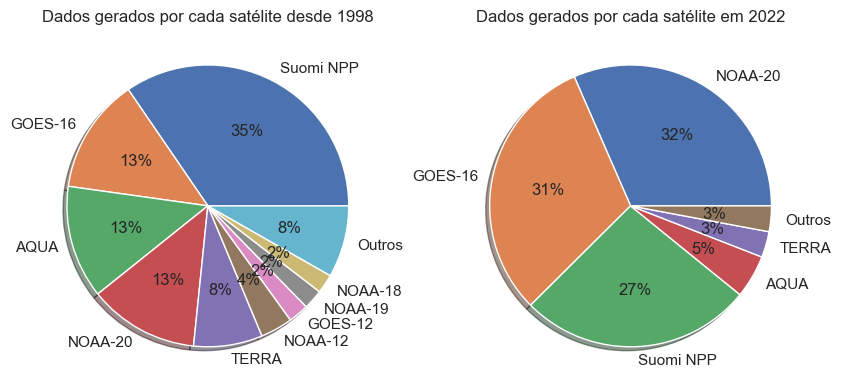
\includegraphics[width=35em]{porcentagem_satelites}
    \end{center}
    \legend{Fonte: O Autor}
    \label{fig:porcentagem_satelites}
\end{figure}

Saber em quais momentos os satélites passam também é importante para a análise. 
Os satélites polares passam duas vezes por dia no Brasil, variando o local 
exato da passagem de acordo com as características de sua órbita. Pela  
figura \ref{fig:tempo_medidas_satelites} é possível comprovar esse comportamento 
empiricamente, em que os 5 primeiros gráficos, que representam dados gerados por 
satélites polares, apresentam dois picos durante um período de 24 horas. Já para o  
caso dos geoestacionários (GOES-16), que ficam fixos em relação a uma posição 
na Terra, não se observou o mesmo padrão. 
[P6. Mostrar gráficos que indicam as horas das coletas] \par

\begin{figure}
    \caption{Amostragem por tempo de cada satélite}
    \begin{center}
        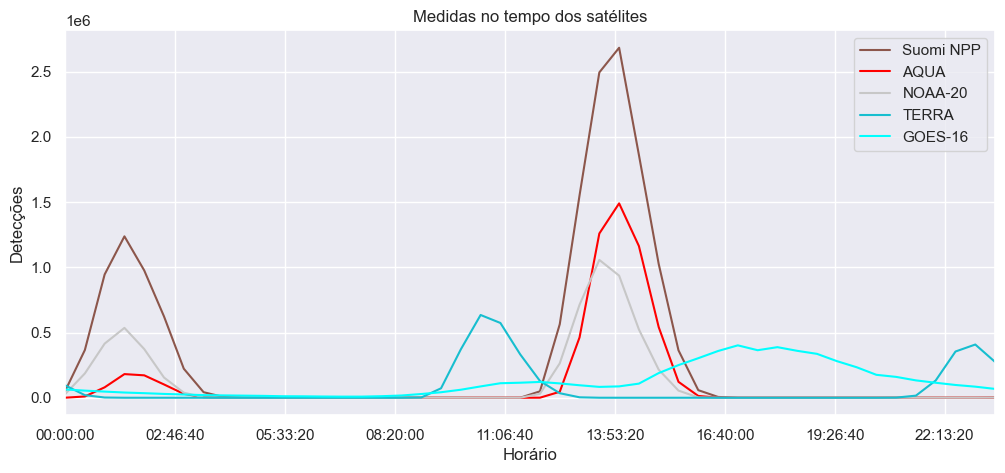
\includegraphics[width=35em]{tempo_medidas_satelites}
    \end{center}
    \legend{Fonte: O Autor, agrupando os dados de queimadas}
    \label{fig:tempo_medidas_satelites}
\end{figure}

Com os dados do \url{https://celestrak.org/} foi possível traçar a rota 
exata de cada satélite de interesse em um dia específico, apresentado na figura 
\ref{fig:orbita2022-08-10}. 
\par

\begin{figure}
    \caption{Órbita dos satélites no dia 10 de agosto de 2022}
    \begin{center}
        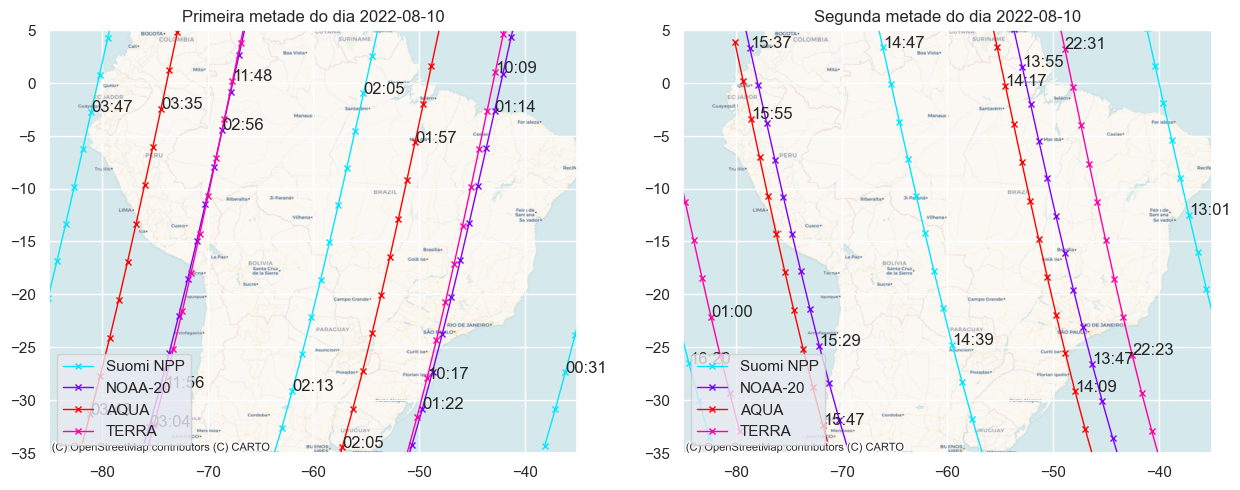
\includegraphics[width=35em]{orbita2022-08-10}
    \end{center}
    \legend{Fonte: O Autor}
    \label{fig:orbita2022-08-10}
\end{figure}

\section{O que os dados gritam}

P1. Fazer análise preliminar dos dados gerando alguns gráficos \par
P2. Gráficos geral do brasil com os focos de queimadas totais \cite{geographicDataSciencePython} \par


\chapter{Aprofundando a análise dos dados}

aqui a gente mostra que é válido usar esses dados para analises aprofundadas

\section{Densidade e Centrografia}

P1. Verificar densidade e centrografia: tendências, dispersão, extensão \par

\section{Validade dos dados}

Precisamos verificar que os dados seguem algum padrão para ser possível
user eles para tomadas de decisões (garantir que não é aleatório) 
\cite[Point Pattern Analysis]{geographicDataSciencePython} \par

\section{Padronizando os dados por satélite}

P1. Verificar relação entre dados dos diferentes satélites (se possível) e talvez restringir a análise apenas ao satélite de referencia se for identificado que são basicamente equivalentes \par

\chapter{Correlações}

P1. Levantar variáveis que podem influenciar nas queimadas \par
P2. Variáveis humanas: influencia da agricultura, pecuária, 
urbanização, áreas de preservação, reservas indígenas \par
P3. Variáveis naturais: Clima, ondas solares, períodos de chuvas/secas \par



\bibliographystyle{abntex2-alf}
\bibliography{biblio}

\end{document}
